\subsection{Quadratics Inequalities}
\begin{definition}[Quadratics Inequalities]
  A math sentence with a squared term where the highest power is $2$, and it uses signs like $>$, $<$, $\ge$, or $\le$ instead of a $=$ sign.

  
  The standard forms is as follows:


  $a \ne 0$
  \begin{itemize}
  \item $ax^2 + bx + c > 0$
  \item $ax^2 + bx + c < 0$
  \item $ax^2 + bx + c \ge 0$
  \item $ax^2 + bx + c \le 0$
  \end{itemize}
\end{definition}

\begin{example}[Quadratics Inequalities]
  \hfill
  \begin{enumerate}
  \item $x^2 - 3x - 10 \le 0$ \\
    $x^2 - 3x - 10 = 0$ \\
    \begin{center}
      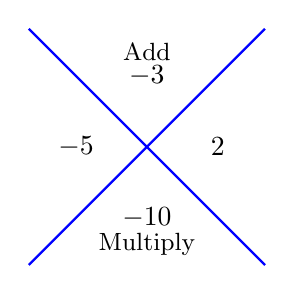
\begin{tikzpicture}[scale=1.5, auto, >=stealth]
	\draw[thick, blue] (-1, 1) -- (1, -1);
	\draw[thick, blue] (-1, -1) -- (1, 1);
	\node at (0, 0.6) {$-3$};
	\node at (0, -0.6) {$-10$};
	\node at (-0.6, 0) {$-5$};
	\node at (0.6, 0) {$2$};
	\node at (0, 0.6) [above=2pt] {\small Add};
	\node at (0, -0.6) [below=2pt] {\small Multiply};
      \end{tikzpicture}
    \end{center}
    $(x - 5)(x + 2) = 0$ \\
    $x - 5 = 0 \land x + 2 = 0$ \\
    $x = 5 \land x = -2$ \\
    $[-2,5]$ \\
    $(0)^2 - 3(0) - 10 \le 0$ \\ 
    $v(-10 \le 0) = \top $
  \item $2x^2 < 5x + 3$ \\
    \textbf{Note: }We can actually change the inequalities and still get the same answer. \\
    $2x^2 - 5x - 3 < 0$ \\
    \begin{center}
      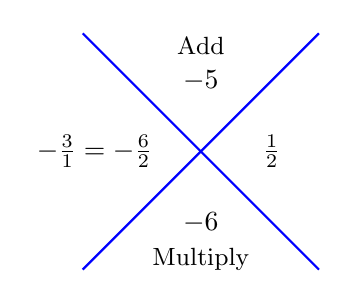
\begin{tikzpicture}[scale=1.5, auto, >=stealth]
	\draw[thick, blue] (-1, 1) -- (1, -1);
	\draw[thick, blue] (-1, -1) -- (1, 1);
	\node at (0, 0.6) {$-5$};
	\node at (0, -0.6) {$-6$};
	\node at (-0.9, 0) {$-\frac{3}{1} = -\frac{6}{2}$};
	\node at (0.6, 0) {$\frac{1}{2}$};
	\node at (0, 0.6) [above=6pt] {\small Add};
	\node at (0, -0.6) [below=6pt] {\small Multiply};
      \end{tikzpicture}
    \end{center}
    $x = 3 \land x = -\frac{1}{2}$ \\
    $\left(-\frac{1}{2}, 3\right)$ \\
    $2(0) - 5(0) - 3 < 0$ \\
    $v(-3 < 0) = \top$
  \item $x(x + 1) > 20$ \\
    $x^2 + x > 20$ \\
    $x^2 + x - 20 > 0$ \\
    \begin{center}
      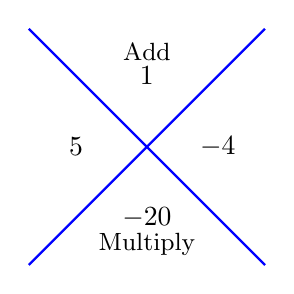
\begin{tikzpicture}[scale=1.5, auto, >=stealth]
	\draw[thick, blue] (-1, 1) -- (1, -1);
	\draw[thick, blue] (-1, -1) -- (1, 1);
	\node at (0, 0.6) {$1$};
	\node at (0, -0.6) {$-20$};
	\node at (-0.6, 0) {$5$};
	\node at (0.6, 0) {$-4$};
	\node at (0, 0.6) [above=2pt] {\small Add};
	\node at (0, -0.6) [below=2pt] {\small Multiply};
      \end{tikzpicture}
    \end{center}
    $(x + 5)(x - 4)  0$ \\
    $x = -5 \land x = 4$ \\
    $(-\infty, -5) \cup (4, \infty)$ \\
    $(0)^2 + (0) - 20 > 0$ \\
    $v(-20 > 0) = \bot$
  \item $4x^2 + 9 < 6x$ \\
    $4x^2 - 6x + 9 < 0$ \\
    $x = \frac{-(-6) \pm \sqrt{(-6)^2 - 4(4)(9)}}{2(4)}$ \\
    $x = \frac{6 \pm \sqrt{36 - 144}}{8}$ \\
    \textbf{Note: }This parabola has \textbf{NO} $x$-axis. \\
    $4(0)^2 - 6(0) + 9 < 0$ \\
    $v(9 < 0) = \bot$
  \end{enumerate}
\end{example}
